\section{PSpice Simulation}
The D-Latch circuit was built using an inverting CMOS structure and four NAND gates, using two PMOS and two NMOS transistors each. The circuit is shown in figure \ref{fig:spicecircuit}.
\begin{figure}[h!]
	\centering
	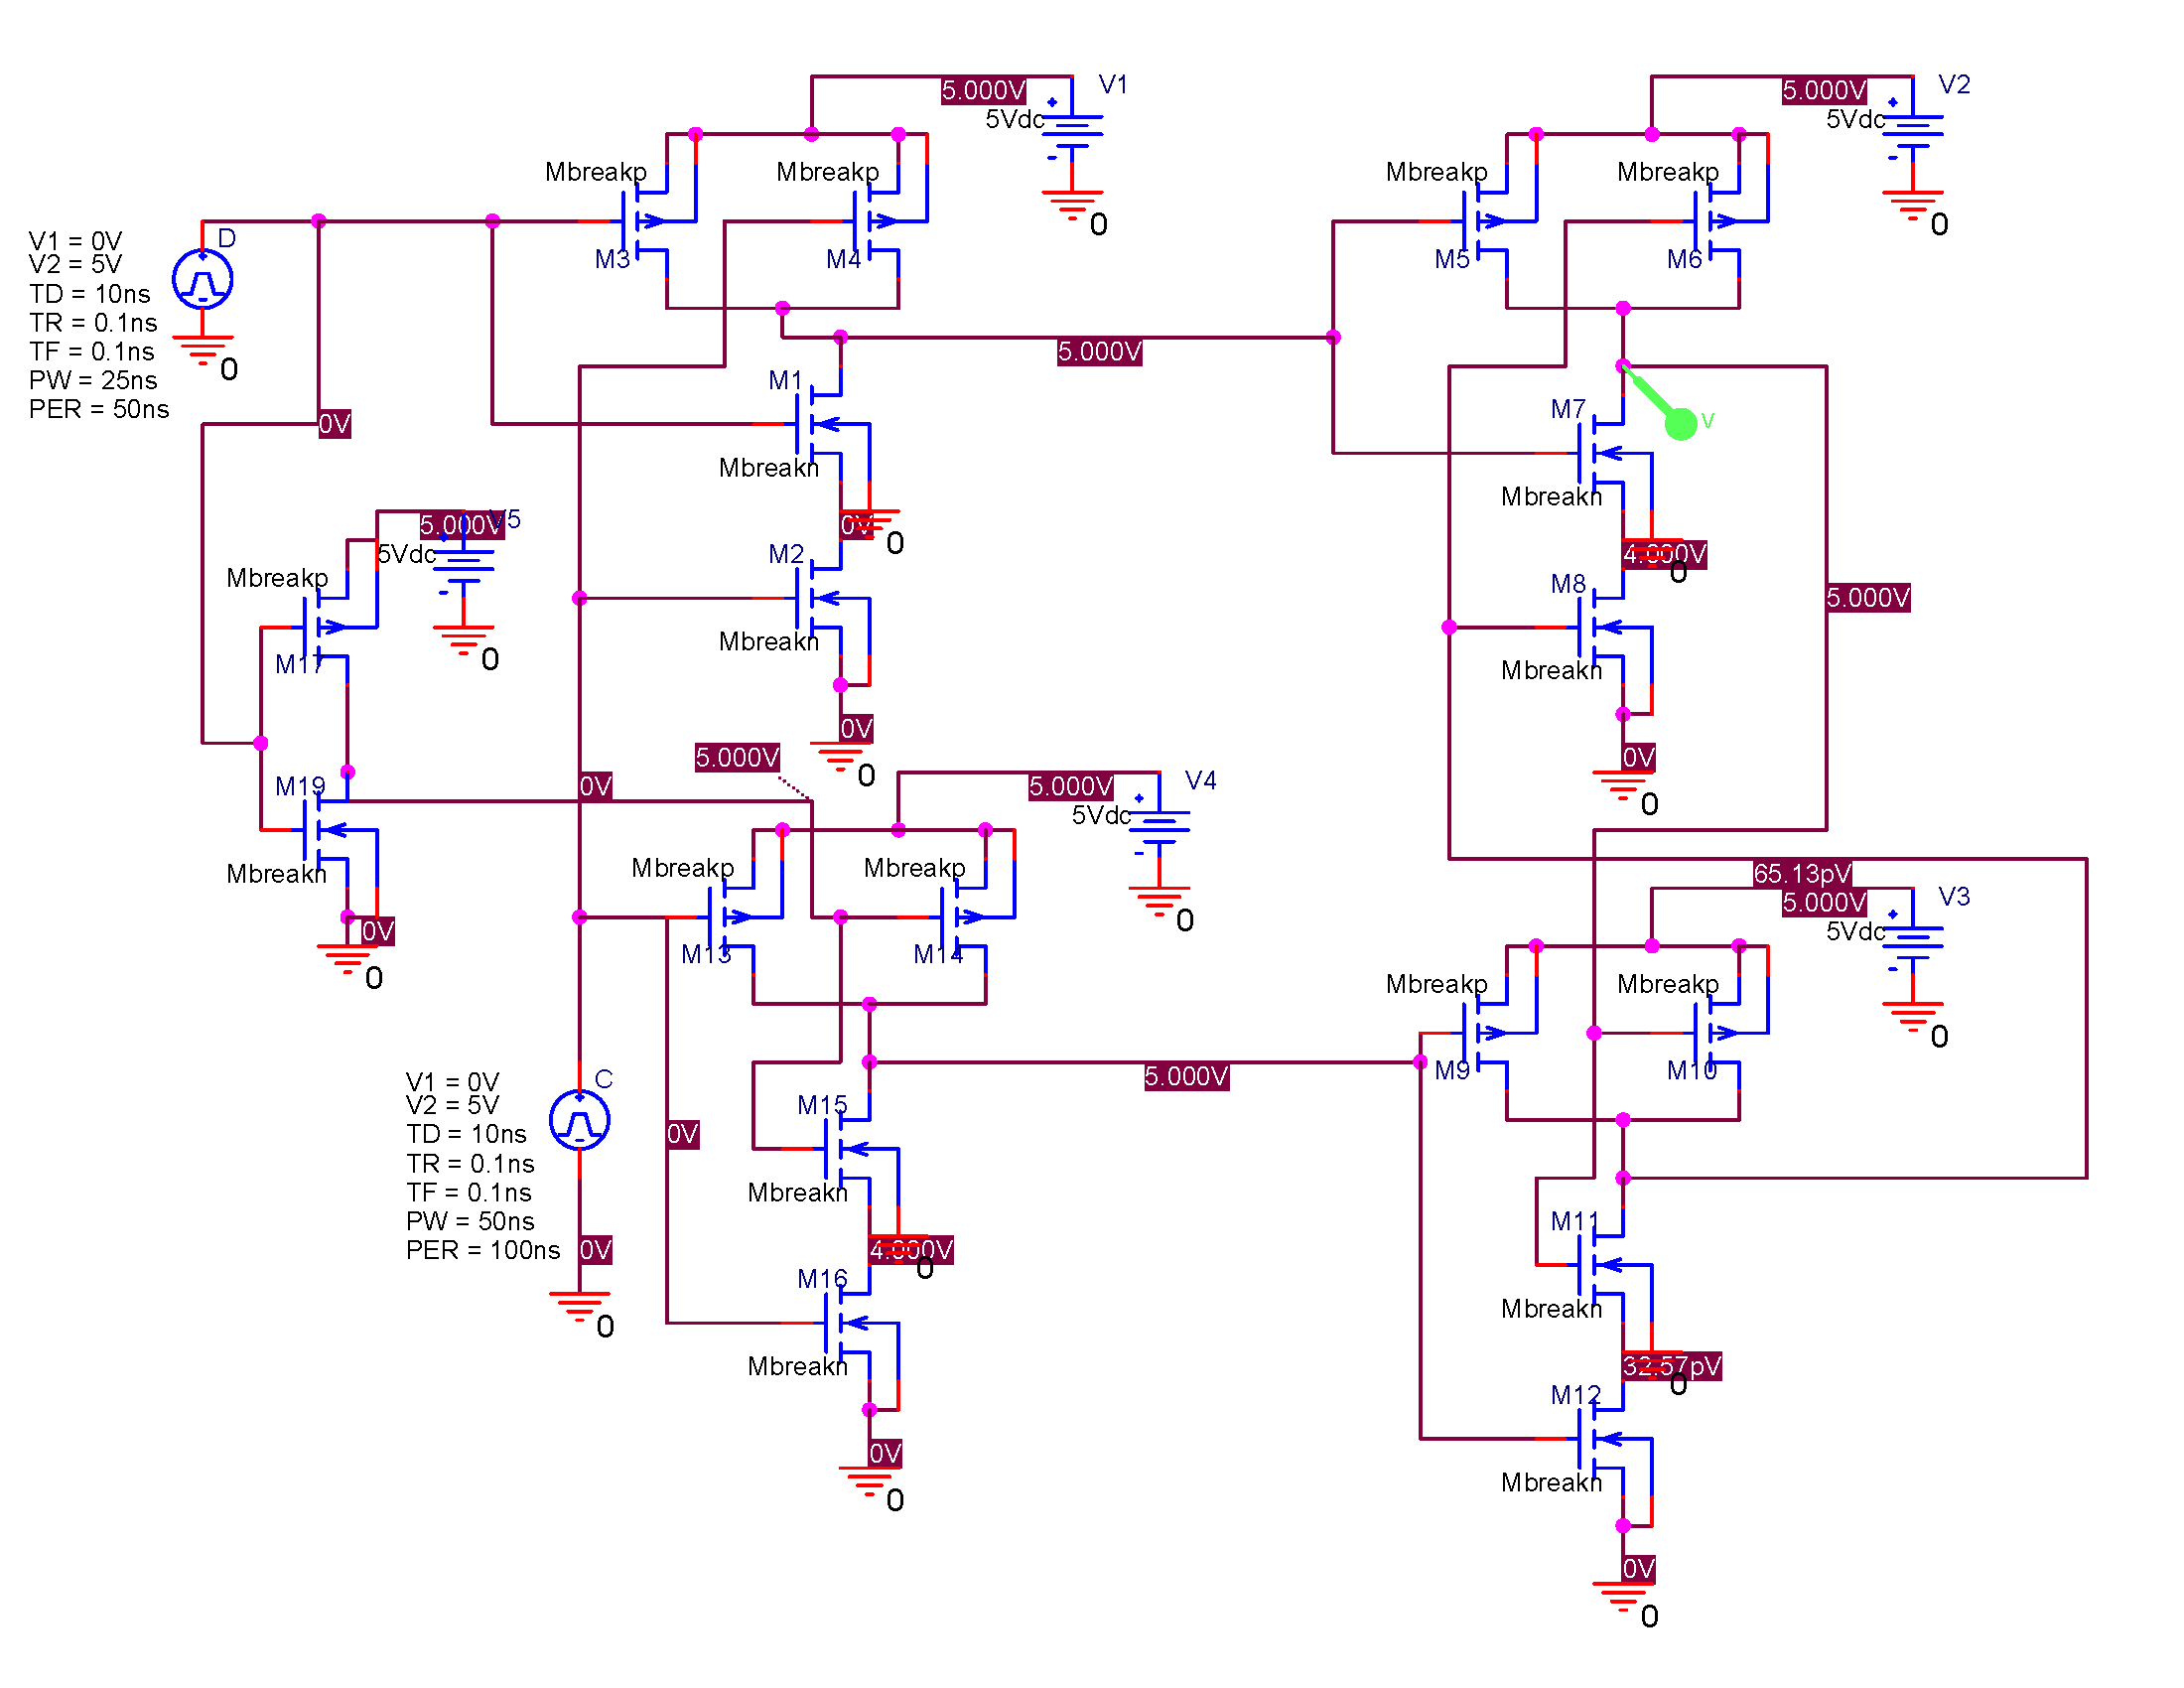
\includegraphics[width=1\linewidth]{../images/spice_circuit}
	\caption{The D-Latch circuit model for PSpice simulation.}
	\label{fig:spicecircuit}
\end{figure}

Our assumption is that when the control input is high the value of the input, D, will be stored as the output value. This value will change with D; however, when the control input is low the value of the output cannot be changed. For example, if we have D high and C high, the output will be high, but if we then change C to low, then the value of D before the change will be stored as the output value until C is brought high again. The behavior of the D-Latch is shown in the FSM in figure \ref{fig:dlatch_fsm}.


\FloatBarrier

\begin{figure}[h!]
	\centering
	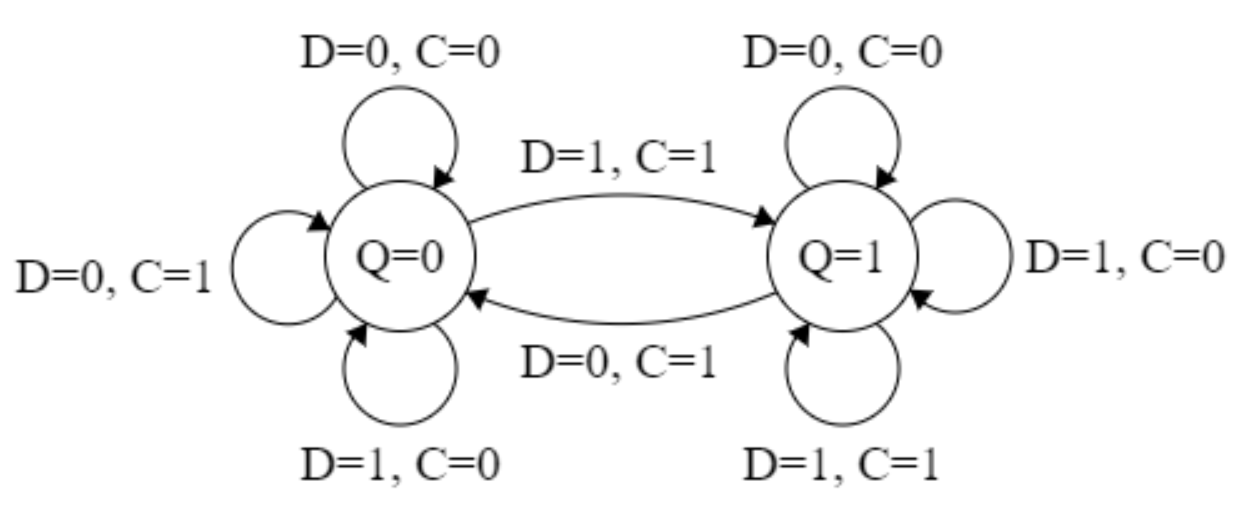
\includegraphics[scale=0.75]{../images/dlatch_fsm}
	\caption{The behavior of a D-Latch.}
	\label{fig:dlatch_fsm}
\end{figure}

\FloatBarrier





The results of all the simulations were consistent with the assumed behavior of the D-Latch circuit. In figure \ref{fig:spec_sim} it is shown that when the control input is high the value of input D is stored at the output Q, and when the control input is low the value of D is passed to the output Q. For this simulation the input and control input the settings in figure \ref{fig:supplys} were used. These values were supplied in the lab specification document.

There is a small spike that occurs when D is becoming high while C is becoming low. This is believed to be due to propagation delays that occur while the values are changing; however, these effects quickly die out and the values returns to the expected behavior.

\FloatBarrier

\begin{figure}[h!]
	\centering
	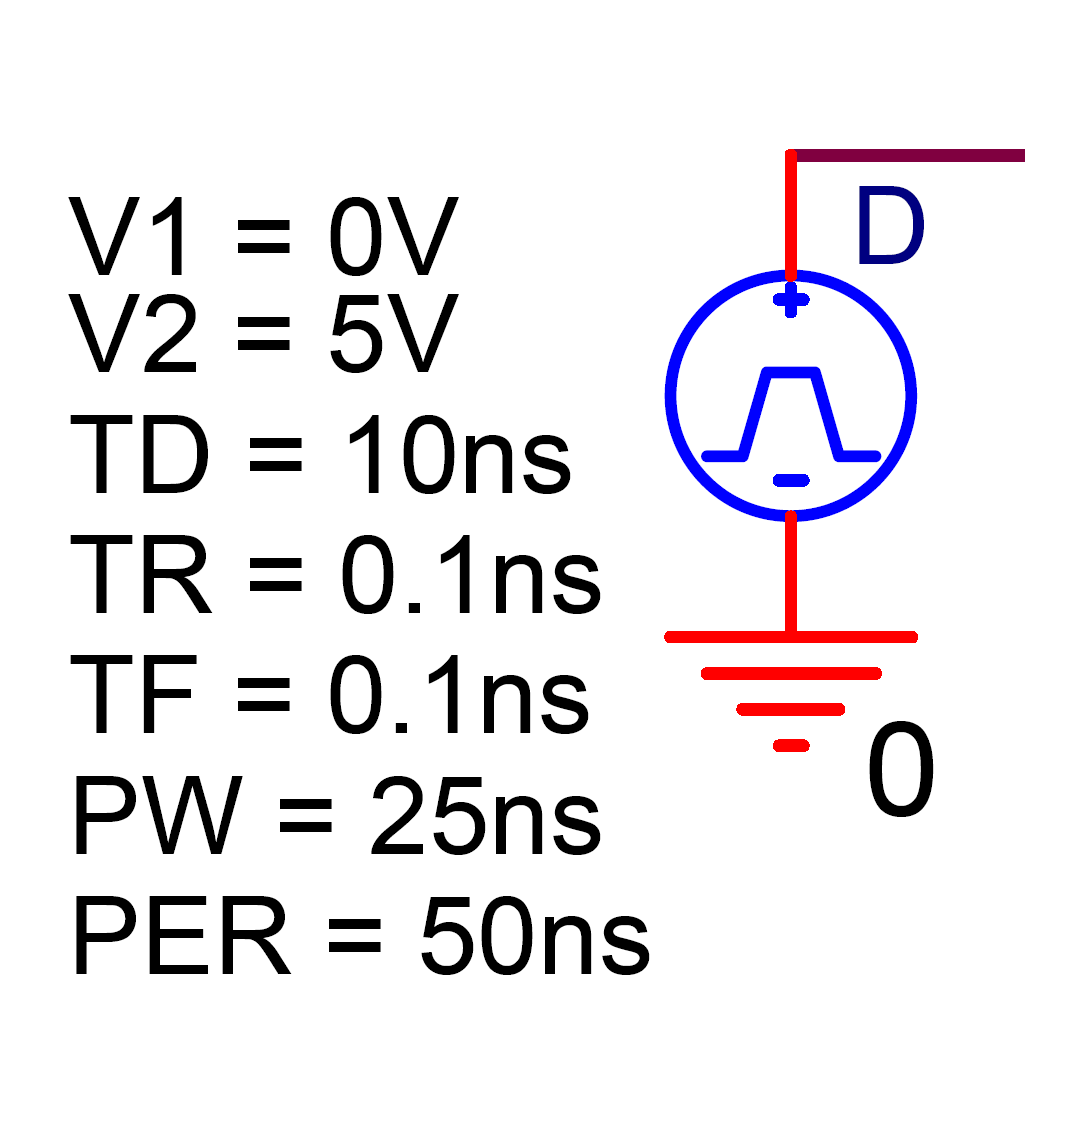
\includegraphics[width=0.4\textwidth]{../images/D_supply}
	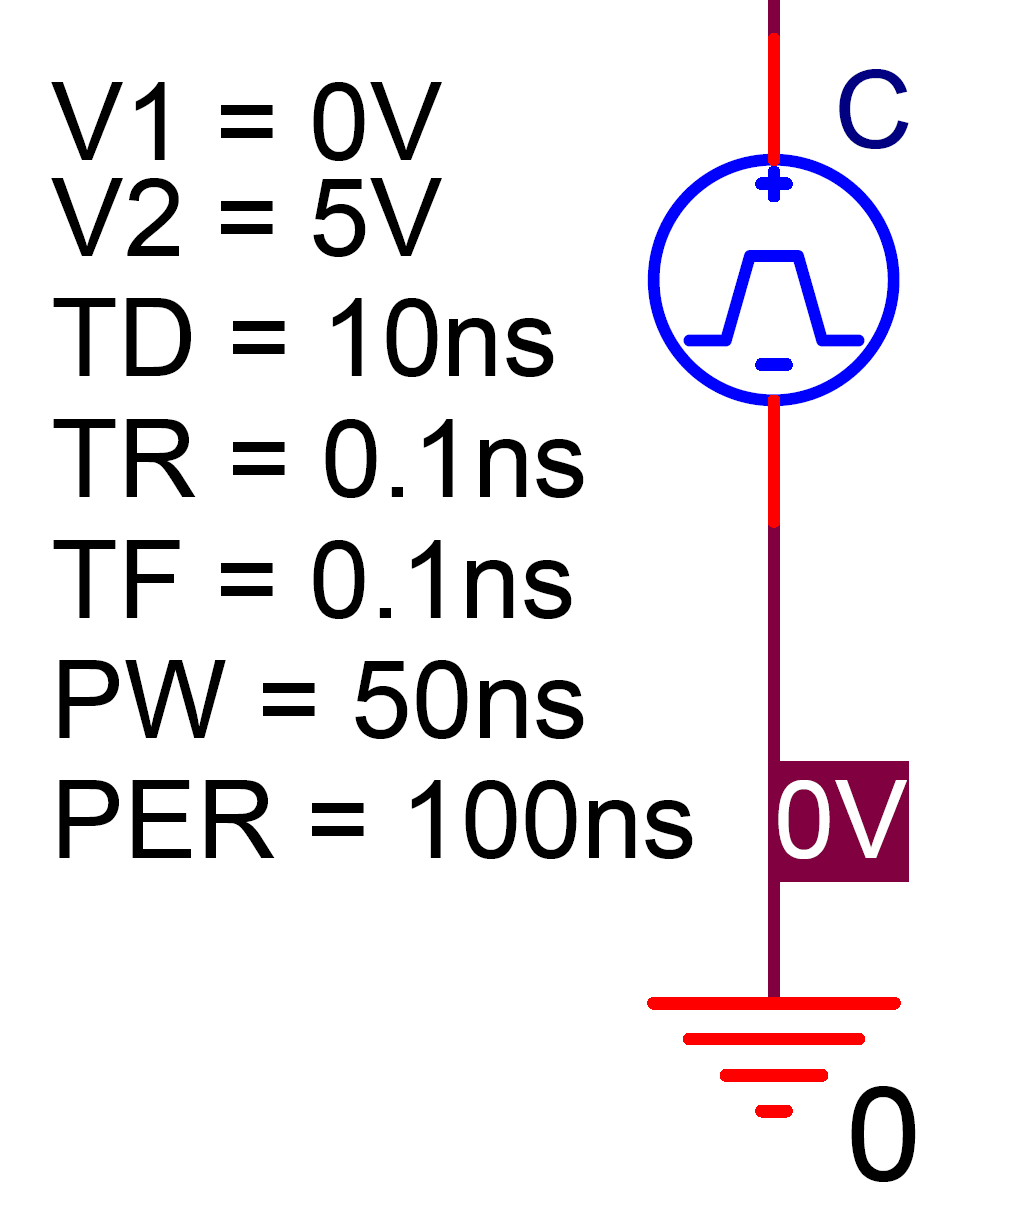
\includegraphics[width=0.4\textwidth]{../images/C_supply}
	\caption{The simulated input (left) and the simulated control input.}
	\label{fig:supplys}
\end{figure}

\FloatBarrier

\FloatBarrier

\begin{figure}[h!]
	\centering
	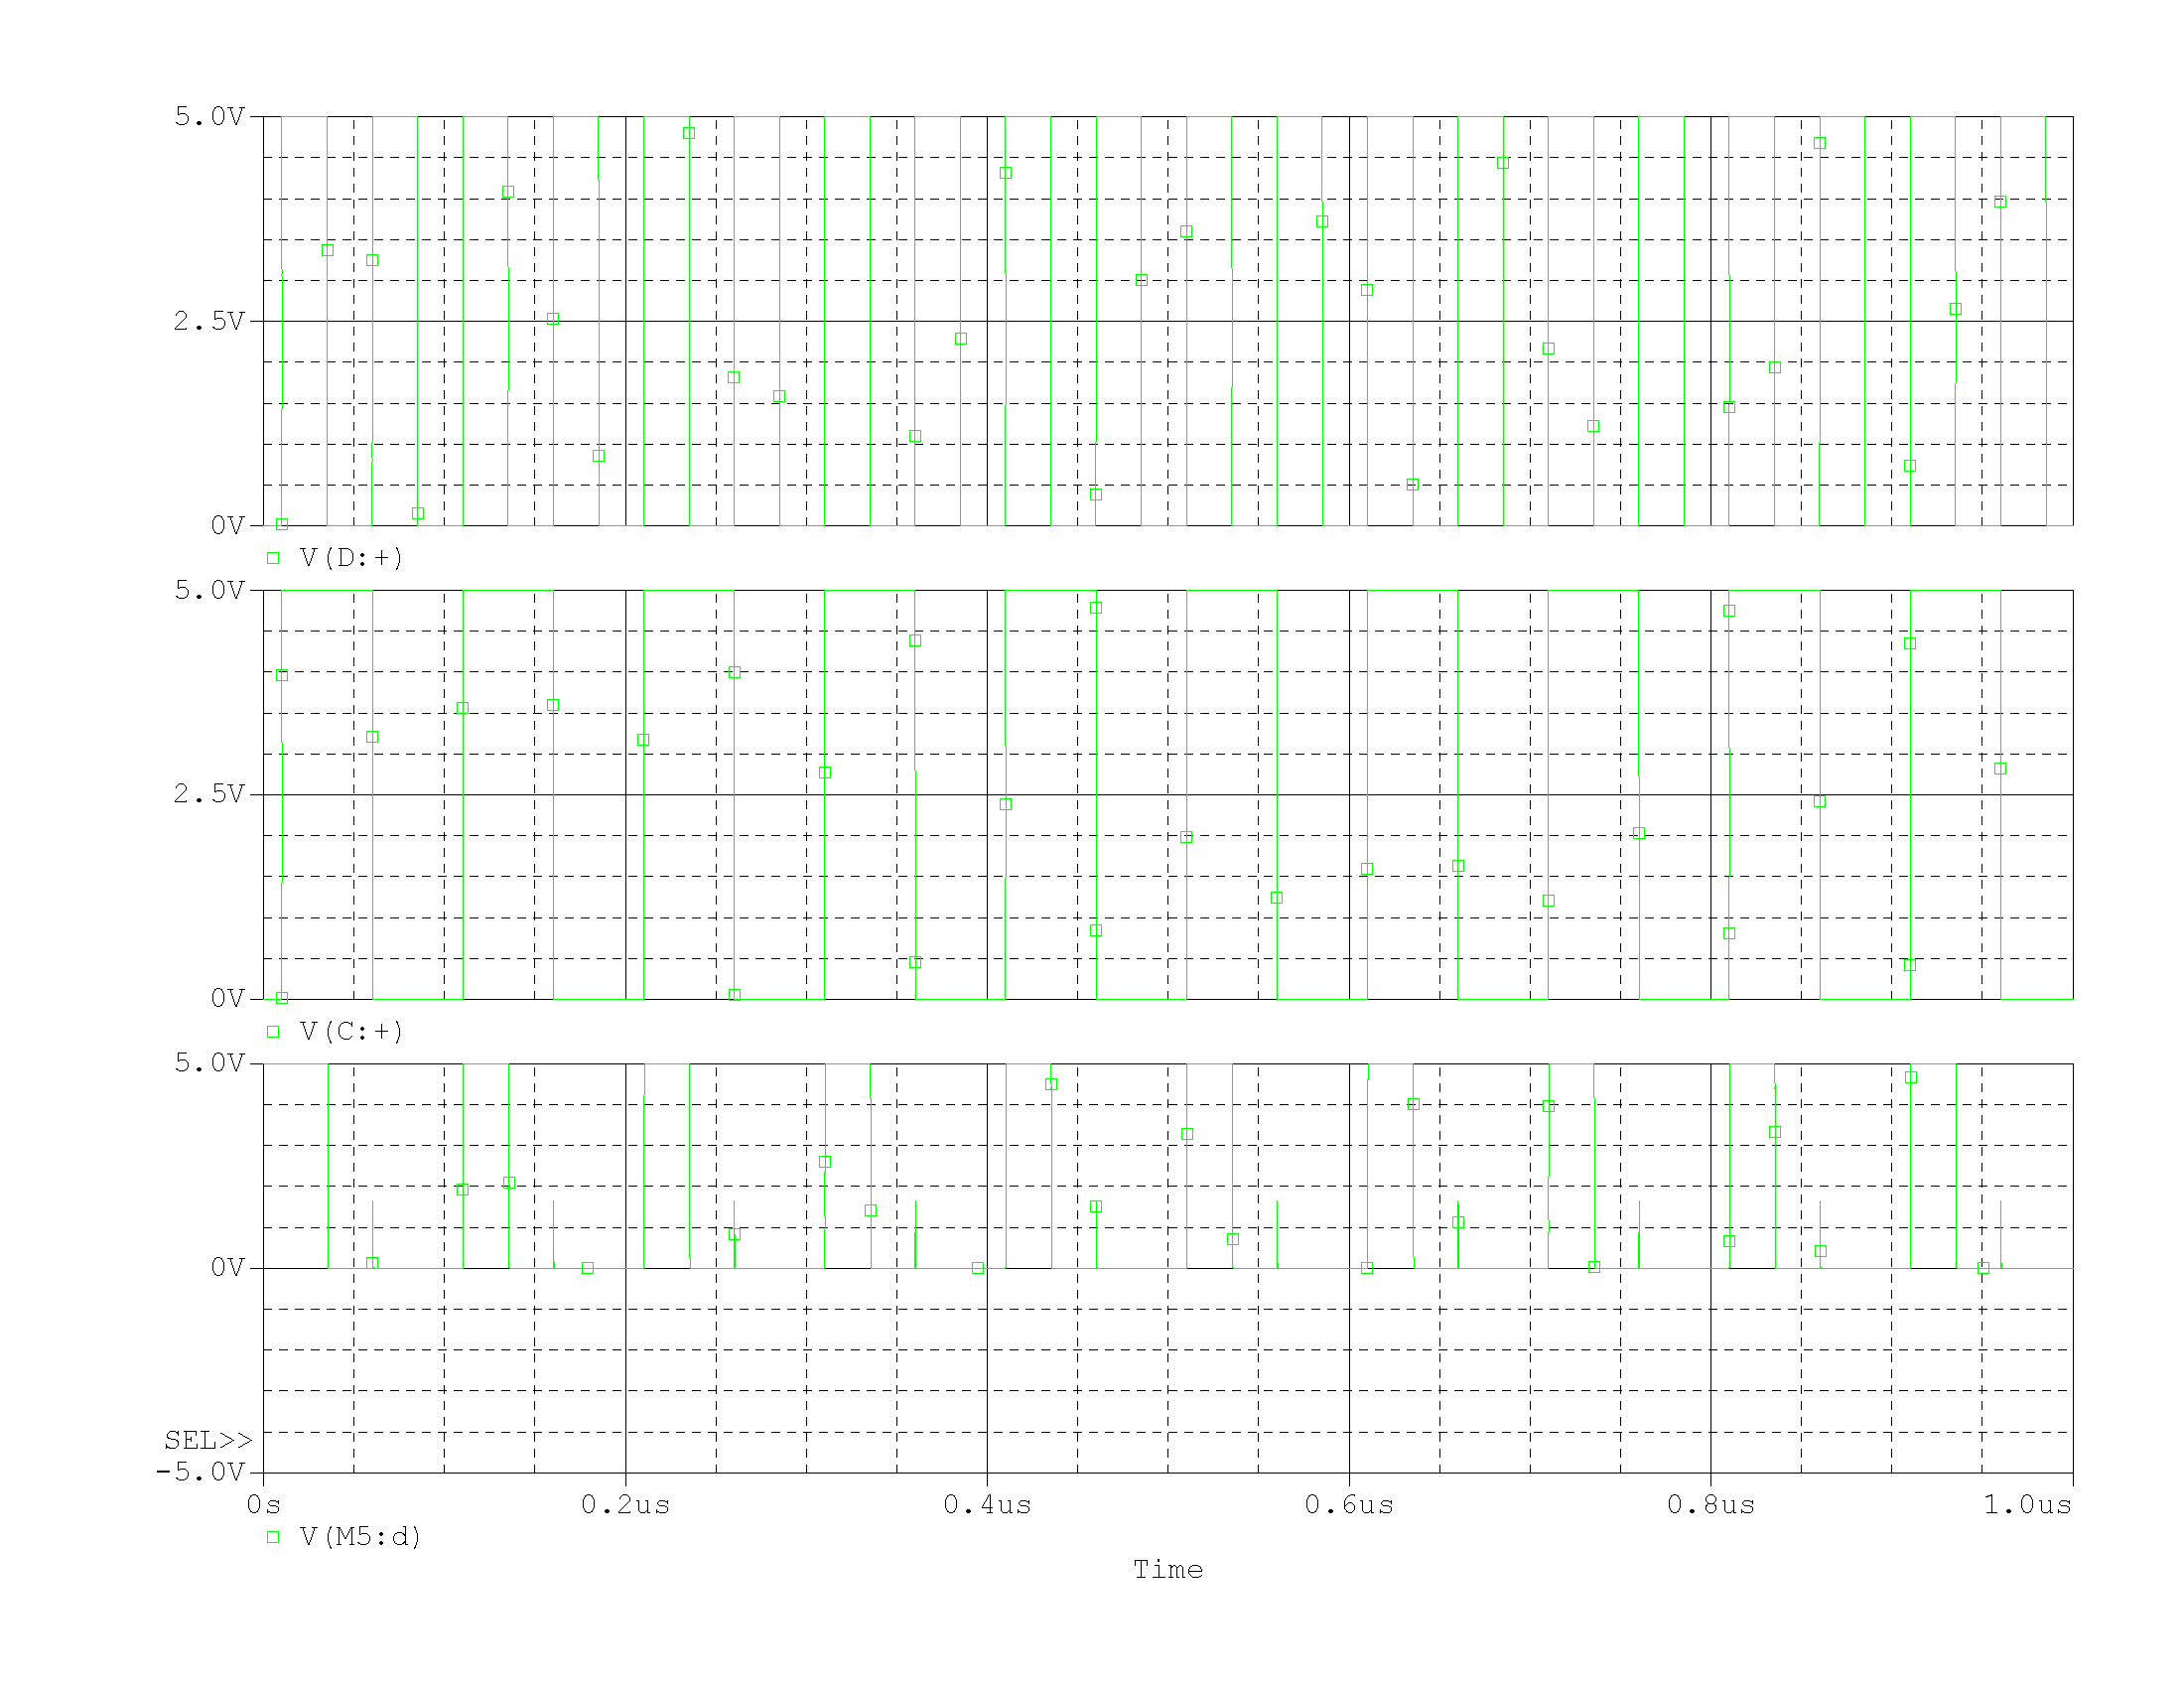
\includegraphics[width=1\linewidth]{../images/spec_sim}
	\caption{The simulation results of our D-Latch, using inputs from figure \ref{fig:supplys}.}
	\label{fig:spec_sim}
\end{figure}

\FloatBarrier
